\documentclass[12pt, a4paper]{article}
\usepackage[utf8]{inputenc}
\usepackage[IL2]{fontenc}
\usepackage[czech]{babel}
\usepackage{graphicx}

\begin{document}
\begin{figure}[h!]
\centering

\includegraphics[bb= 0 0 820 445 , width=75mm]{favlogo.jpg}
\end{figure}

{\centering
{\huge Hledání min}\\[1em]
{\large KIV/DB2}\\[11,5cm]
}

\begin{tabular}{l r}
student: & Radek VAIS\\
os. číslo: & A17N0093P\\
mail: & vaisr@students.zcu.cz\\
datum: & 16.5.2018\\
\end{tabular}

\thispagestyle{empty}
\newpage

%========================================
%========================================
%========================================
%========================================
%========================================
\section{Zadání} %=====================================================================================================

Navrhněte a vytvořte relační databázi pro hraní známé počítačové hry Hledání min. Protože bude řešena pouze databázová vrstva aplikace, snažte se co nejvíce programových rutin uložit do databáze a také zajistěte jejich automatickou aktivaci při nastalé události.
Herní oblast má zpravidla tvar obdélníku, ve kterém se nachází několik min. Velikost oblasti a počet min v ní definuje obtížnost hry. Hráč si může vybrat jednu ze tří předdefinovaných obtížností nebo si může definovat obtížnost vlastní. Úkolem hráče je odkrýt všechna pole oblasti, která nejsou zaminována. Hráči se bude od začátku hry měřit čas, aby bylo možné dosažené výsledky porovnávat. Po odkrytí libovolného pole (hráčem nebo databází) může nastat jedna z těchto událostí:

\begin{itemize}
\item Hráč šlápl na minu. Hra končí neúspěchem a výsledek se zaznamená do databáze.
\item Bylo odkryto poslední pole, na kterém není mina. Hra končí úspěchem, protože zbylá neodkrytá pole obsahují miny. Také v tomto případě se výsledek uloží do databáze.
\item Bylo odkryto pole, které je volné a nesousedí s žádným zaminovaným polem. V tomto případě databáze automaticky odkryje všechna sousední pole – ty mají společný min. jeden vrchol.
\end{itemize}

Pro snazší hraní si může hráč označovat ta pole, o kterých si myslí, že jsou zaminovaná. K tomuto rozhodnutí mu pomohou čísla již odkrytých polí, která určují, s kolika zaminovanými poli toto pole sousedí. Takto označené pole nelze odkrýt, ale toto označení lze kdykoliv zrušit.

K realizaci využijte prostředky Oracle SQL dostupné na serveru students.kiv.zcu.cz.

\subsection{Požadavky na datbázové objekty}

Výsledná práce bude obsahovat alespoň následující databázové objekty.

\subsubsection{Tabulky}
\begin{itemize}
\item OBTIZNOST - Každá hra musí mít definovanou obtížnost. Buď bude vybrána předdefinovaná, nebo si hráč definuje obtížnost vlastní. Hodnoty parametrů vlastní obtížnosti se ukládají do tabulky OBLAST. Tabulka bude obsahovat obtížnosti dle originální hry.
\item OMEZENI - Každá vlastní obtížnost musí splňovat jistá omezení. Např. počet řádků či sloupců nesmí být menší než 9 a větší než 100. Také je vhodné pohlídat, aby počet rozmístěných min v zaminované oblasti nebyl příliš velký, např. nepřekročil 40 procent její velikosti.
\item OBLAST - Každá zaminovaná oblast je vytvořená podle vlastní obtížnosti a obsahuje její hodnoty. Hráč má za úkol oblast od min vyčistit.
\item POLE - Elementární část zaminované oblasti definovaná svými souřadnicemi, která může nést minu nebo informaci, s kolika zaminovanými poli sousedí.
\item MINA - Hráčem označovaná pole, o kterých si myslí, že jsou zaminovaná.
\item TAH - Hráčem odkrývaná pole v zaminované oblasti. Ke každému tahu se bude automaticky ukládat časová značka, kdy byl tah vykonán.
\item STAV - Číselník obsahující, v jakých stavech se hra může vyskytovat. Stavy mohou být tyto: rozehraná, úspěšně ukončená, neúspěšně ukončená.
\item HRA - Průběžně aktualizované informace o probíhající hře. Obsahuje časové značky prvního a naposledy provedeného tahu, počet označených min a stav hry.
\end{itemize}

\subsubsection{Databázové pohledy}

\begin{itemize}
\item CHYBNE\_MINY - Seznam polí v zaminované oblasti, které byly chybně označené jako zaminované. Nabízí data pro všechny oblasti.
\item VITEZOVE - Výsledková tabulka her, které byly úspěšně dokončené. Měla by ukazovat parametry obtížnosti (rozměry oblasti a počet min) dané hry a také dobu hraní hry (rozdíl časových značek posledního a prvního tahu).
\item PORAZENI - Výsledková tabulka her, které byly neúspěšně dokončené. Měla by navíc (oproti pohledu VITEZOVE) ukazovat, kolik min bylo správně odhaleno.
\item OBLAST\_TISK - Zobrazení celé zaminované oblasti včetně odkrytých polí a (hráčem) označených min. Každý řádek oblasti bude zobrazen voláním funkce RADEK\_OBLASTI.
\end{itemize}

\subsubsection{Procedury}

\begin{itemize}
\item ZAMINUJ\_OBLAST - Položení min na (náhodná) místa v definované oblasti. Počet zaminovaných polí je uloženo v tabulce OBLAST.
\item SPOCITEJ\_OBLAST - Pro každé nezaminované pole v oblasti spočítá, s kolika zaminovanými poli sousedí. Do tabulky POLE ukládá hodnoty z intervalu 0 až 8.
\item ODKRYJ\_POLE - Rekurzivní procedura, která pro právě odkryté pole, které nesousedí s žádným zaminovaným polem, odkryje všechna jeho neodkrytá sousední pole.
\item OZNAC\_MINY - Po úspěšném dohrání hry budou dosud neodkrytá pole označená jako zaminovaná, tj. vloží odpovídající záznamy do tabulky MINA.
\end{itemize}

\subsubsection{Funkce}

\begin{itemize}
\item SPATNY\_PARAMETR - Oznámí, zda hodnota parametru vlastní obtížnosti porušila definovaná omezení.
\item RADEK\_OBLASTI - Vrátí řetězec znaků ukazující aktuální podobu daného řádku zaminované oblasti.
\item ODKRYTA\_MINA - Oznámí, že právě odkryté pole skrývá minu, což znamená neúspěšný konec hry.
\item MNOHO\_MIN - Nelze označit více zaminovaných polí, než kolik min je v oblasti.
\item VYHRA - Počet neodkrytých polí se rovná počtu min, které se v oblasti nachází. Pokud ano, hra končí úspěchem.
\end{itemize}

\subsubsection{Triggery}

Triggery se starají o automatické činnosti v databázi. Jedná se o:

\begin{itemize}
\item hlídání hodnot parametrů vlastní obtížnosti (volání funkce SPATNY\_PARAMETR).
\item kopírování hodnot parametrů obtížnosti pro aktuální oblast, pokud byla zvolena základní obtížnost.
\item zaminování nastavené oblasti (volání procedury ZAMINUJ\_OBLAST) a očíslování polí této oblasti (volání procedury SPOCITEJ\_OBLAST).
\item volání automatických kontrol (volání funkcí ODKRYTA\_MINA a VYHRA) a případně akcí (volání procedury ODKRYJ\_POLE) při odkrytí pole.
\item zabránění odkrytí již odkrytého pole.
\item hlídání počtu polí označených jako zaminované (volání funkce MNOHO\_MIN).
\item zabránění označení pole jako zaminované, které je již takto označeno nebo je odkryté.
\item průběžnou aktualizaci hry po každém jejím tahu.
\item označení min, pokud hra skončila úspěšně (volání procedury OZNAC\_MINY).
\item zabránění odkrytí pole, pokud hra (neúspěšně) skončila.
\item zabránění odkrytí pole, které je hráčem označené jako zaminované.
\end{itemize}


%====================================================================================================================================================
\newpage

\section{Popis řešení}

Význam databázových objektů je dostatečně popsán již v zadání, to ale dostatečně nepostihuje vztahy mezi objekty a jejich vlastnosti. Tyto informace jsou zobrazeny v ERA modelu na Obrázku 1. 


\begin{figure}[h!]
\centering
\label{fig:era}
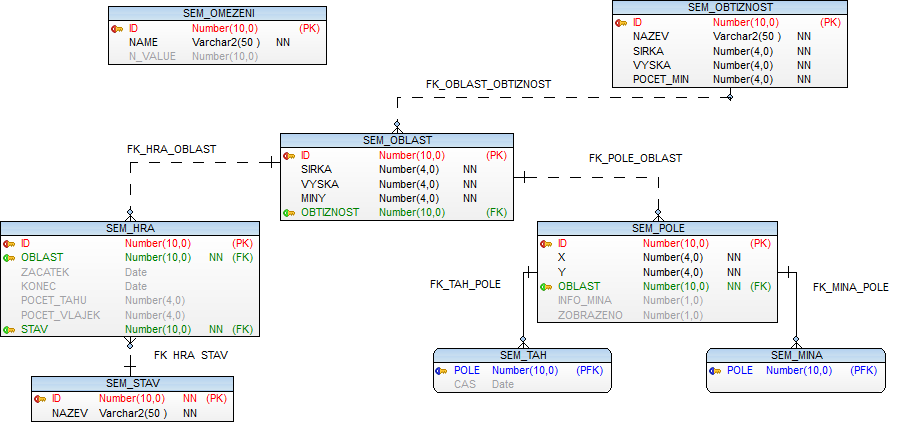
\includegraphics[bb= 0 0 908 423 , width=150mm]{ERA.png}
\caption{ERA model pro hru Hledání min}
\end{figure}

\subsection{Pohledy}

Součástí databázového řešení jsou čtyři pohledy na uložená data. Základní pohledy "vítězové", "poražení" dále jsou k dispozici pohledy "chybné miny" a "oblast tisk".

Pohledy vítězové a poražení poskytují informace o dohraných hrách. Pohled vždy transformuje data tabulky "hra" a "oblast" do uživatelsky přívětivých hodnot (přepočet délky hry). 

\begin{verbatim}
CREATE OR REPLACE VIEW sem_porazeni 
AS
    SELECT o.sirka AS sirka, o.vyska AS vyska, o.miny AS miny
        , h.pocet_tahu AS pocet_tahu
        , (h.konec - h.zacatek)*(24)  AS doba_hry_hodiny
        ,(h.konec - h.zacatek)*(24 * 60) AS doba_hry_minuty
        ,(h.konec - h.zacatek)*(24 * 60 * 60) AS doba_hry_sekundy
    FROM sem_hra h
    LEFT JOIN sem_oblast o ON h.oblast = o.id
    WHERE h.stav = 4
;
\end{verbatim}

Dalším připraveným pohledem je "oblast tisk". Tento pohled využívá funkce pro tisk jednotlivých řádků oblastí. Pohled obsahuje data pro zobrazení řádků všech oblastí. Zde je zásadním prvkem použití DISTINCT selectu pro zvolení unikátních řádků jednotlivých oblastí.

\begin{verbatim}
CREATE OR REPLACE VIEW SEM_OBLAST_TISK AS
	SELECT DISTINCT(y), OBLAST
		, MINESWEEPER.RADEK_OBLASTI(oblast, y) AS RADEK
	FROM sem_pole
	ORDER BY y ASC
;
\end{verbatim}

Data pro jednotlivé oblasti pak získáme jednoduchým selectem například:
\begin{verbatim}
SELECT radek FROM OBLAST_TISK WHERE oblast = 74;
\end{verbatim}

Pohled "chybné miny" pracuje obdobně jako oblast tisk. Pomocí pohledu lze zobrazit pole, která jsou označeny jako mina a zároveň minu nenesou.

\subsection{Procedury a funkce}

Připravené databázové procedury jsou rozděleny do dvou balíků "Minesweeper" a "Minesweeper\_automation". Balík "Minesweeper" obsahuje procedury rozhraní hry (např. zaloz\_hru, oblast\_tisk, mina, tah\ldots). Package "Minesweeper\_automation" pak obsajuje procedury automaticky spouštěné triggery nebo procedurami rozhraní. Balík "Minesweeper\_automation" obsahuje následující funkce obsluhující hru:

\begin{itemize}
\item ZAMINUJ\_OBLAST - Položí miny do oblasti   
\item SPOCITEJ\_OBLAST - Spočítá a nastaví hodnoty nápověd pro hledání min.
\item SPOCITEJ\_POLE - Spočítá počet min na sousedních polích. 
\item VYTVOR\_POLE - Vytvoří entity pro pole oblasti.
\item ODKRYJ\_POLE - Odkryje pole, pokud nesousedí s minou odkryje všechna sousední.
\item VYHRA - Kontroluje, zda hra dosáhla stvu výhry.
\item PROHRA - Kontroluje, zda hra dosáhla stavu prohry.
\item ZOBRAZ\_OBLAST - Automaticky zobrazí všechna pole v oblasti.
\item OZNAC\_MINY - Automaticky označí všechny miny ve zvolené oblasti vlajkou. 
\item MNOHO\_MIN - Kontroluje počet vlajek v oblasti.
\item UKONCENA\_HRA - Kontroluje, zda zvolená oblast je ukončená.   
\item SPATNY\_PARAMETR - Slouží ke kontrole parametrů vlkádaných do tabulky oblast.

\end{itemize} 



Podrobně se zaměříme na dvě vybrné funkce. Základem přípravy hry je funkce "Spocitej\_pole", která slouží k získání počtu sousedních zaminovaných oblastí. Pomocí vnitřního selectu funkce získá počet sousedících min, který následně vrátí jako výsledek funkce. Tato funkce je použita při stavbě hry, pro uložení informací o minách pomocí procedury zaminuj oblast.

\begin{verbatim}
   FUNCTION SPOCITEJ_POLE( an_id_oblast IN NUMBER
                        ,an_x       IN NUMBER
                        ,an_y     IN NUMBER)
    RETURN NUMBER
    IS
        vn_miny_info NUMBER;
    BEGIN
        SELECT info_mina INTO vn_miny_info
           FROM sem_pole WHERE x = an_x
            AND y = an_y AND oblast = an_id_oblast;
        IF vn_miny_info = 9 THEN
            NULL;
            -- do nothing only jump to end of if
        ELSE
            vn_miny_info := 0;
            SELECT COUNT(id)
            INTO vn_miny_info 
              FROM sem_pole 
              WHERE x IN (an_x - 1, an_x , an_x + 1) 
              AND y IN (an_y - 1, an_y , an_y + 1) 
              AND oblast = an_id_oblast
              AND info_mina = 9;
        END IF;
        RETURN vn_miny_info;
    END SPOCITEJ_POLE;
\end{verbatim} 

Procedura odkryj pole slouží k odkrývání oblastí polí, které nesousedí s minou. Jde o rekurzívní proceduru, která postupně odkryje všechna pole nesousedící s minou a jejich sousedící okolí.

\begin{verbatim}
    PROCEDURE ODKRYJ_POLE(an_pole_id IN NUMBER)
    IS
        vn_miny NUMBER;
        vn_oblast NUMBER;
        vn_x NUMBER;
        vn_y NUMBER;
    BEGIN
        UPDATE sem_pole SET zobrazeno = 1 WHERE id = an_pole_id;
        SELECT info_mina, oblast,
        	 x, y 
        INTO vn_miny, vn_oblast,
         vn_x, vn_y
        FROM sem_pole WHERE id = an_pole_id;
        IF vn_miny = 0 THEN
            FOR pole IN ( SELECT info_mina, id 
                            FROM sem_pole 
                            WHERE x IN (vn_x - 1, vn_x , vn_x + 1) 
                            AND y IN (vn_y - 1, vn_y , vn_y + 1) 
                            AND oblast = vn_oblast
                            AND zobrazeno = 0)
            LOOP
                ODKRYJ_POLE(pole.id);
            END LOOP;
        END IF;
    END ODKRYJ_POLE;
\end{verbatim} 
   

\subsection{Triggery}

Součástí databázového řešení jsou triggery, které vytvářejí odvozené položky, upravují data a kontrolují integritu databáze. Řešení obsahuje následující triggery:

\begin{itemize}
\item T\_BI\_SEM\_HRA\_ID - automaticky nastavuje ID vytvářených her.
\item T\_AD\_SEM\_MINA\_REMOVED - spouští reakci na odstranění vlajky (kontrola počtu a úprava tabulky hry).
\item T\_AI\_SEM\_MINA\_PLACED - spouští reakci na vložení vlajky.
\item T\_AI\_SEM\_OBLAST - spouští vytvoření závislých entit oblasti.
\item T\_AI\_SEM\_TAH\_PLAYED - spouští odkrytí polí, aktualizaci hry a kontrolu koncového stavu hry. 
\item T\_BI\_SEM\_MINA\_COUNT - ověřuje počet vlajek v oblasti.
\item T\_BI\_SEM\_OBLAST - provádí kopii hodnot standardních obtížností.
\item T\_BI\_SEM\_OBLAST\_ID - automaticky nastavuje ID vytvářených oblastí.
\item T\_BI\_SEM\_OBLAST\_PARAM - kontroluje parametry vytvářené oblasti.
\item T\_BI\_SEM\_POLE\_ID - utomaticky nstavuje ID vytvářených polí.
\item T\_BI\_SEM\_TAH - nastavuje aktuální čas tahu a kontroluje, zda hra není v koncovém stavu.
\item T\_BI\_SEM\_TAH\_SHOWED - kontroluje, zda pole není odhaleno. 
\end{itemize} 

Podrobně se zaměříme jen na dva příklady. Trigger, který slouží k automatickému odrývání polí a využívá proceduru "ODKRYJ\_Pole" je "trigger\_ai\_sem\_tah\_played". Tento trigger také upravuje statistiky hry do které byl zahrán tah. 

\begin{verbatim}
CREATE OR REPLACE TRIGGER trigger_ai_sem_tah_played
AFTER INSERT 
ON sem_tah
FOR EACH ROW
DECLARE 
    vn_oblast_id NUMBER;
BEGIN
   MINESWEEPER_AUTOMATION.ODKRYJ_POLE(:new.pole);
   
   -- urči id oblasti do které byl zahrán tah
   SELECT o.id INTO vn_oblast_id FROM sem_pole p, sem_oblast o
   WHERE o.id = p.oblast
   AND p.id = :new.pole;
   
   -- první tah aktualizuje zacatek hry
   UPDATE sem_hra set zacatek = :new.cas, stav = 2 
   WHERE oblast = vn_oblast_id AND zacatek IS NULL;
   
   -- další tahy zvyšují počítadlo hry
   UPDATE sem_hra set pocet_tahu = (COALESCE(pocet_tahu, 0) + 1 ) 
   WHERE oblast = vn_oblast_id;
   
   MINESWEEPER_AUTOMATION.PROHRA(vn_oblast_id);
   MINESWEEPER_AUTOMATION.VYHRA(vn_oblast_id);
END
;
\end{verbatim}

Ukázkou triggeru, který slouží ke kontrole integrity dat je trigger\_bi\_sem\_oblast\_param:

\begin{verbatim}
CREATE OR REPLACE TRIGGER trigger_bi_sem_oblast_param
	BEFORE INSERT
 	ON sem_oblast
 	FOR EACH ROW
BEGIN
    MINESWEEPER_AUTOMATION.SPATNY_PARAMETR(:new.sirka
    						, :new.vyska, :new.miny);
END;
\end{verbatim}

\section{Ovládání}

\subsection{Nasazení}

Pro nasazení databázové logiky slouží scripty uložené ve složce src. V této složce je umístěn soubor README.txt, který obsahuje pořadí spouštění jednotlivých SQL skriptů pro vytvoření všech objektů a naplnění základními daty (např. definice obtížností). Vytvářející scripty vytvoří databázové entity definované zadáním s prefixem "SEM\_".

\subsection{Hra}

Pro snadné ovládání hry je připraven soubor \textit{game.sql}, který obsahuje připravené anonymní PL/SQL bloky pro volání jednotlivých funkcí rozhraní balíku Minesweeper. Průběh hry je vypisován do DBMS konzole, případně je uživateli zobrazena výjimka popisující porušení pravidel hry.

Hráč určuje, do jaké oblasti na jaké souřadnice chce šlápnout a tedy pole odhalit. Rozehraná hra po několika krocích může vypadat následujícím způsobem:

\begin{verbatim}
TAH  (15, 1, 1);
TAH  (15, 1, 9);
MINA (15, 4, 6);
OBLAST_TISK (15);
                      1 o o o o o o o o
                      o o o o o o o o o
                      o o o o o o o o o
                      1 1 1 o o o o o o
                      - - 1 o o o o o o
                      - - 1 ? o o o o o
                      - - 1 2 o o o o o
                      - - - 1 1 1 1 o o
                      - - - - - - 1 o 2
\end{verbatim}

Číslo určuje počet sousedních min, malé \texttt{o} označuje zakryté pole a \texttt{?} uživatelskou vlajku. Pomlčkou (\texttt{-}) je označeno pole, které nesousedí s minou.

\section{Závěr}

V rámci této semestrální práce byl vytvořen ERA model hry Hlednání min, 8 entitních tabulek, 4 pohledy na uložená data, 14 triggerů kontrolujících integritu databáze  a 12 funkcí a procedur, které jsou volány z triggerů, nebo z rozhraní "Minesweeper".

Databázové řešení slouží k simulaci hry Hledání min s využitím prostředků Oracle SQL.

\end{document}